%!TEX program = xelatex
\documentclass[cn,hazy,blue,14pt,screen,device=normal]{elegantnote}
\usepackage{multirow}
\usepackage{enumitem}
\usepackage{caption}

\title{物理层; 概述}

\author{李聪聪}
\institute{3GPP TS 38.201 V15.0.0}

\version{1.0}
\date{\zhtoday}

\usepackage{array}

\begin{document}

\maketitle

\newpage
\tableofcontents
\newpage

\section{层 1 概述}
\subsection{与其他层的关系}
\subsubsection{协议架构}
 本规范中描述的无线电接口涵盖了用户设备(UE)和网络之间的接口。 无线接口由第1层,第2层和第3层组成。
 
 \begin{figure}[!hbp]
 	\centering
 	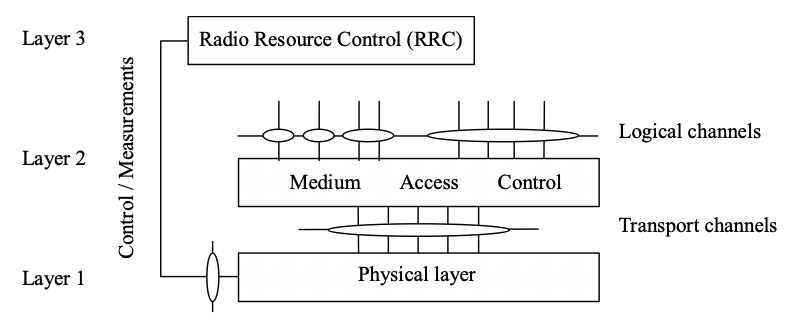
\includegraphics{Figure1Layers}
 	\caption{无线接口协议架构}
    \label{Figure1Layers}
 \end{figure}


如图 \ref{Figure1Layers} 所示,物理层连接着媒体访问控制层(Medium Access Control, MAC, 层 2)和无线资源控制层(Radio Resource Control, RRC, 层 3)。 不同层之间的圆圈表示服务访问点(Service Access Points, SAPs)。

物理层为 MAC 层提供了传输信道,而 MAC 层为 RRC 层提供了逻辑信道。不同逻辑信道上传输不同的数据,而不同的传输信道则规定了信息该如何通过空口进行传输。

物理层相关的规范参考 TS 38.200 系列。

MAC 层和 RRC 层相关规范参考 TS 38.300 系列。

\subsubsection{物理层为高层所提供的服务}
物理层为高层提供数据传输服务。MAC 层通过传输信道将需要发送的数据传递给物理层。详细内容可参考 3GPP TS 38.202: "NR; Services provided by the physical layer"。

\subsection{层 1 概述}
\subsubsection{多路访问}
NR物理层的多址方案基于具有循环前缀(CP)的正交频分复用(OFDM)。 对于上行链路,还支持带有CP的离散傅立叶变换扩频OFDM(DFT-s-OFDM)。 为了支持成对和非成对频谱的传输,同时使用了频分双工(FDD)和时分双工(TDD)。

为了使 NR 的物理层适应各种频谱分配,规定物理层以资源块(Resource Block, RB)为单位使用频谱资源。一个资源块包含 12 个相同间隔的子载波。

一个无线帧的持续时间为 10ms,包含 10 个子帧,子帧的持续时间为 1ms。每个子帧包括一个或多个时隙(slot),每个时隙包括 12/14 个符号(symbol)。关于帧结构的更多内容参考 3GPP TS 38.202: "NR; Services provided by the physical layer"。

\subsubsection{物理信道和调制}
下行链路的物理信道包括以下几个:

\begin{itemize}[leftmargin=2cm]
	\item 物理下行链路共享信道(PDSCH)
	\item 物理下行链路控制信道(PDCCH)
	\item 物理广播信道(PBCH)
\end{itemize}

上行链路的物理信道包括以下几个:
\begin{itemize}[leftmargin=2cm]
	\item 物理随机接入信道(PRACH)
	\item 物理上行链路共享信道(PUSCH)
	\item 物理上行链路控制信道(PUCCH)
\end{itemize}

此外,还定义了主同步信号(Primary Synchronization Signal, PSS)、辅同步信号(Secondary Synchronization Signal, SSS)和参考信号(Reference Signal, RS)。

调制方案如下所示:

\begin{table}[!hbp]
	\resizebox{\textwidth}{12mm}{ 
		\begin{tabular}{|c|c|c|c|c|c|c|c|c|c|}
		\hline
         	& \multicolumn{4}{c|}{OFDM}                                                                         & \multicolumn{5}{c|}{DFT-s-OFDM}                             \\ \hline
			Downlink & \multirow{2}{*}{QPSK} & \multirow{2}{*}{16QAM} & \multirow{2}{*}{64QAM} & \multirow{2}{*}{256QAM} &                             &      &       &       &        \\ \cline{1-1} \cline{6-10} 
			Uplink   &                       &                        &                        &                         & $\pi / 2$-BPSK & QPSK & 16QAM & 64QAM & 256QAM \\ \hline
		\end{tabular}}
	\caption{调制方案}
	\label{modulation}
\end{table}

\subsubsection{信道编码}
NR 根据传输信道和控制信息的不同,选用不同的信道编码方案。基于传输信道的不同,编码方案的选择如表 \ref{ChannelCodingBasedOnTrCHs} 所示。基于控制信息的不同,编码方案的选择如表 \ref{ChannelCodingBasedOnControlInfo} 所示。关于信道编码的更多内容可参考 3GPP TS 38.212: "NR; Multiplexing and channel coding"。

\begin{table}[!hbp]
	\centering
	\setlength{\tabcolsep}{25mm}
	\begin{tabular}{|c|c|}
	\hline
	传输信道   & 编码方案                  \\ \hline
	UL-SCH & \multirow{3}{*}{LDPC} \\ \cline{1-1}
	DL-SCH &                       \\ \cline{1-1}
	PCH    &                       \\ \hline
	BCH    & Polar code            \\ \hline
	\end{tabular}
	\caption{ 不同传输信道的编码方案 }
	\label{ChannelCodingBasedOnTrCHs}
\end{table}

\begin{table}[!hbp]
	\centering
	\setlength{\tabcolsep}{25mm}
	\begin{tabular}{|c|c|}
	\hline
	控制信息                 & 编码方案       \\ \hline
	DCI                  & Polar Code \\ \hline
	\multirow{2}{*}{UCI} & Block Code \\ \cline{2-2} 
                     & Polar Code \\ \hline
	\end{tabular}
	\caption{ 不同控制信息的编码方案 }
	\label{ChannelCodingBasedOnControlInfo}
\end{table}


\subsubsection{物理层流程}
物理层包括以下流程:
\begin{itemize}[leftmargin=2cm]
	\item 小区搜索
	\item 功率控制
	\item 上行同步和上行定时控制
	\item 随机接入相关流程
	\item HARQ 相关流程
	\item 波束管理和 CSI 相关流程
\end{itemize}

NR 通过在频域、时域以及功率上对物理层资源的控制,提供了对干扰协调的支持。

\subsubsection{物理层测量}
无线电特性由 UE 和网络完成测量,并上报给高层。测量包括以下内容:
\begin{itemize}[leftmargin=2cm]
	\item 频率内和频率间切换的测量
	\item RAT 间切换的测量
	\item 定时测量 
	\item RRM 测量 
\end{itemize}

RAT 间切换的测量用于支持 E-UTRA 的切换。

\section{物理层规范文档结构}
\subsection{概览}
物理层规范文档结构如图 \ref{DocumentStructureOfPhysicalLayer} 所示:
 \begin{figure}[!htbp]
 	\centering
 	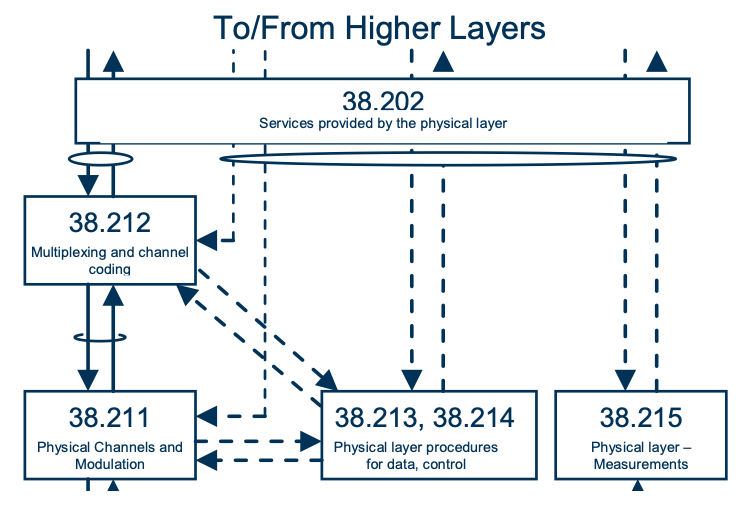
\includegraphics{DocumentStructureOfPhysicalLayer}
 	\caption{物理层规范结构}
    \label{DocumentStructureOfPhysicalLayer}
 \end{figure}

\subsection{TS 38.201: 物理层概述}

TS 38.201: Physical layer; General description 为物理层概述文档,包括以下内容:
\begin{itemize}[leftmargin=2cm]
	\item 层 1 文档简介(TS 38.200 系列)
	\item 从哪里获取信息
\end{itemize}

\subsection{TS 38.202: 物理层所提供的服务}
TS 38.202: Physical layer services provided by the physical layer 描述了物理层所提供的服务,具体包括以下内容:
\begin{itemize}[leftmargin=2cm]
	\item 物理层的服务和功能
	\item UE 的物理层模型
	\item 同步物理信道和 SRS 的并行传输
	\item 由物理层提供的测量
\end{itemize}

\subsection{TS 38.211: 物理信道和调制}
TS 38.211: Physical channels and modulation 描述了物理信道的特性、物理层信号的生成和调制。具体包括以下内容:
\begin{itemize}[leftmargin=2cm]
	\item 定义上行和下行物理信道
	\item 帧结构和物理资源
	\item 调制映射(BPSK, QPSK 等)
	\item OFDM 信号的生成
	\item 加扰、调制和上变频
	\item 层映射和预编码
	\item 上行链路和下行链路中的物理共享信道
	\item 上下行参考信号
	\item 物理随机接入信道
	\item 主同步信号和辅同步信号
\end{itemize}

\subsection{TS 38.212: 多路复用和信道编码}
TS 38.212: Multiplexing and channel coding 描述了传输信道和控制信道数据处理,包括复用、信道编码和交织。具体包括以下内容:
\begin{itemize}[leftmargin=2cm]
	\item 信道编码方案
	\item 速率匹配
	\item 上行传输信道和控制信息
	\item 下午传输信道和控制信息
\end{itemize}

\subsection{TS 38.213: 物理层控制流程}
TS 38.213: Physical layer procedures for control 描述了用于控制的物理层流程。具体包括以下内容:
\begin{itemize}[leftmargin=2cm]
	\item 同步流程
	\item 上行功率控制
	\item 随机接入流程
	\item UE 上报控制信息流程
	\item UE 接收控制信息流程
\end{itemize}

\subsection{TS 38.214: 物理层数据流程}
TS 38.214: Physical layer procedures for data 描述了用于数据传输的物理层流程。具体包括以下内容:
\begin{itemize}[leftmargin=2cm]
	\item 功率控制
	\item 物理下行共享信道相关流程
	\item 物理上行共享信道相关流程
\end{itemize}

\subsection{TS 38.215: 物理层测量}
TS 38.215: Physical layer measurements 描述了物理层测量的相关特性。具体包括以下内容:
\begin{itemize}[leftmargin=2cm]
	\item UE/NG-RAN 测量的控制
	\item NR 的测量功能
\end{itemize}

\end{document}
